\chapter{Risultati}
\section{Risultati su challenge Kaggle}
L'approccio proposto negli scorsi capitoli per l'identificazione delle anomalie statiche e dinamiche ha prodotto diversi risultati che andiamo a riportare in questo capitolo, in particolare questo paragrafo è incentrato sul setting sperimentale fornito dal dataset della challenge di Kaggle e le anomalie statiche in esso riscontrate.  
\noindent Tale dataset possedendo un numero molto elevato di istanze è ottimale per capire l'effettiva efficienza ed efficacia dell'approccio proposto sviluppato con il supporto del \textit{Decision Tree Classifier} per l'estrazione delle regole.

I dati dopo un pre-processamento che li porta in scala logaritmica in base dieci, attraverso l'algoritmo di clustering subiscono un processo di divisione da cui risultano essere scomposti in vari cluster. Nel caso di alcuni mesi, risultano essere presenti cluster formati da un solo cliente e per questo segnalati come anomali.

Il dataset così elaborato viene dato interamente in input al \textit{Decision Tree Classifier} per elaborare le regole che vadano a spiegare il comportamento dei clienti ed in particolare ci concentreremo sulla regola estratta per il cliente anomalo. Inoltre, è possibile estrarre anche l'albero creato dalle regole estratte. 

Il quinto mese della challenge di Kaggle è di seguito riportato come esempio dei risultati che possono essere ottenuti tramite l'applicazione dell'approccio. Nella Figura \ref{fig:kaggle} è possibile osservare come al termine del clustering vengano evidenziati due utenti anomali presenti nel mese le cui regole vengono in seguito riportate.

\begin{figure}[H]
    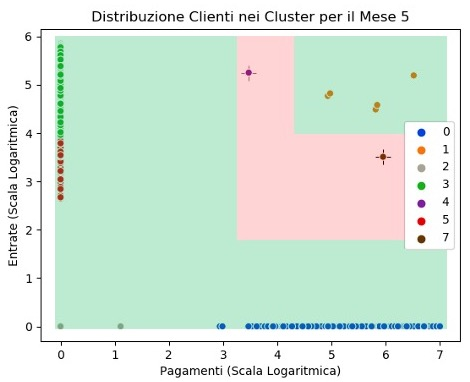
\includegraphics[width=0.7\textwidth]{M5.jpeg}
    \centering
    \caption{Distribuzione dei Clienti per il Mese 5}
    \label{fig:kaggle}
\end{figure}

\noindent L'albero estratto dal \textit{Decision Tree Classifier} viene riportato di seguito in cui vengono segnalate tramite \verb{class:1{ le foglie dove sono situate le anomalie, che corrispondo alle due anomalie visibili nella figura \ref{fig:kaggle}. \\

\begin{center}
\begin{minipage}{6cm}
\begin{Verbatim}[t][fontsize=\small, frame=single]
|--- PAGAMENTI <= 3.47
| |--- class: 0
|--- PAGAMENTI > 3.47
| |--- ENTRATE <= 1.75
| | |--- class: 0
| |--- ENTRATE > 1.75
| | |--- PAGAMENTI <= 4.20
| | | |--- class: 1
| | |--- PAGAMENTI > 4.20
| | | |--- ENTRATE <= 4.00
| | | | |--- class: 1
| | | |--- ENTRATE > 4.00
| | | | |--- class: 0
\end{Verbatim}
\end{minipage}
\end{center}
%\clearpage
\newpage

\noindent Le regole ottenute dal \textit{Decision Tree Classifier} per tutti i cluster del mese vengono di seguito riportate in notazione logaritmica e  in scala reale: \\
\vspace{1cm}

\begin{minipage}{7cm}
\raggedright
\begin{Verbatim}[t][fontsize=\small, frame=single]
Rule 1
Rule: PAGAMENTI <= 2953.173

Rule 3
Rule: PAGAMENTI > 2953.173
Rule: ENTRATE <= 56.877

Rule 5
Rule: PAGAMENTI > 2953.173
Rule: ENTRATE > 56.877
Rule: PAGAMENTI <= 15953.775
\end{Verbatim}
\end{minipage}%
\begin{minipage}{6cm}
\raggedleft
\begin{Verbatim}[t][fontsize=\small, frame=single]
Rule 7
Rule: PAGAMENTI > 2953.173
Rule: ENTRATE > 56.877
Rule: PAGAMENTI > 15953.775
Rule: ENTRATE <= 10014.66

Rule 8
Rule: PAGAMENTI > 2953.173
Rule: ENTRATE > 56.877
Rule: PAGAMENTI > 15953.775
Rule: ENTRATE > 10014.66 
\end{Verbatim}
\end{minipage}%
 \\
\begin{center}
    Regole in scala reale
\end{center}

\vspace{1.3cm}
 
\begin{minipage}{7cm}
\raggedright
\begin{Verbatim}[t][fontsize=\small, frame=single]
Rule 1
Rule: PAGAMENTI <= 3.47

Rule 3
Rule: PAGAMENTI > 3.47
Rule: ENTRATE <= 1.755

Rule 5
Rule: PAGAMENTI > 3.47
Rule: ENTRATE > 1.755
Rule: PAGAMENTI <= 4.203
\end{Verbatim}
\end{minipage}%
\begin{minipage}{6cm}
\raggedleft
\begin{Verbatim}[t][fontsize=\small, frame=single]
Rule 7
Rule: PAGAMENTI > 3.47
Rule: ENTRATE > 1.755
Rule: PAGAMENTI > 4.203
Rule: ENTRATE <= 4.001

Rule 8
Rule: PAGAMENTI > 3.47
Rule: ENTRATE > 1.755
Rule: PAGAMENTI > 4.203
Rule: ENTRATE > 4.001
\end{Verbatim}
\end{minipage}%
 \\
\begin{center}
    \\     Regole in scala logaritmica base 10 \\
\end{center}

\newpage
\noindent Confrontando le regole precedentemente estratte con l'albero ottenuto è possibile identificare nelle regole 5 e 7 le anomalie riscontrate in figura \ref{fig:kaggle}. Queste, riportate sia in notazione logaritmica (nella colonna di sinistra) in base dieci sia in scala reale (nella colonna di destra), verranno fornite all'operatore come spiegazione del comportamento utente nel mese corrente, nel caso specifico il quinto mese della challenge Kaggle.
\vspace{1cm}


\begin{minipage}{7cm}
\raggedright
\begin{Verbatim}[t][fontsize=\small, frame=single]
Rule 5
Rule: PAGAMENTI > 3.47
Rule: ENTRATE > 1.755
Rule: PAGAMENTI <= 4.203
\end{Verbatim}
\end{minipage}%
\begin{minipage}{6cm}
\raggedleft
\begin{Verbatim}[t][fontsize=\small, frame=single]
Rule 5
Rule: PAGAMENTI > 2953.173
Rule: ENTRATE > 56.877
Rule: PAGAMENTI <= 15953.775
\end{Verbatim}
\end{minipage}
\vspace{1cm}


\begin{minipage}{7cm}
\raggedright
\begin{Verbatim}[t][fontsize=\small, frame=single]
Rule 7
Rule: PAGAMENTI > 3.47
Rule: ENTRATE > 1.755
Rule: PAGAMENTI > 4.203
Rule: ENTRATE <= 4.001
\end{Verbatim}
\end{minipage}%
\begin{minipage}{6cm}
\raggedleft
\begin{Verbatim}[t][fontsize=\small, frame=single]
Rule 7
Rule: PAGAMENTI > 2953.173
Rule: ENTRATE > 56.877
Rule: PAGAMENTI > 15953.775
Rule: ENTRATE <= 10014.66
\end{Verbatim}
\end{minipage}




\section{Risultati su dati reali}

I risultati ottenuti utilizzando i dati della challenge Kaggle evidenziano come l'approccio proposto riesca ad isolare persone con comportamenti anomali e faciliti l'estrazione  di regole per descriverne il comportamento.

Avendo inoltre a disposizione una piccola parte di un dataset reale di una banca l'approccio è stato testato su questi ulteriori dati per capire i risultati ottenibili in un contesto sconosciuto. Il mese che prendiamo come riferimento è il mese 6 (Giugno) del 2018, dove sono presenti cinque utenti. Essi sono divisi in clienti (User, U) e aziende (Aziende, A) e dalla Figura \ref{fig:challenge} si può notare, che a fronte dei due cluster presenti nel mese, \verb{A1{ forma un cluster formato solo da se stesso che verrà quindi segnalato come anomalo.

Dal momento che il dataset presenta una numerosità molto ridotta le regole vengono generate su una sola metrica perché sufficiente a spiegare il comportamento dell'utente, in questo caso la metrica  è \verb{Min_amount{.

\begin{figure}[H]
    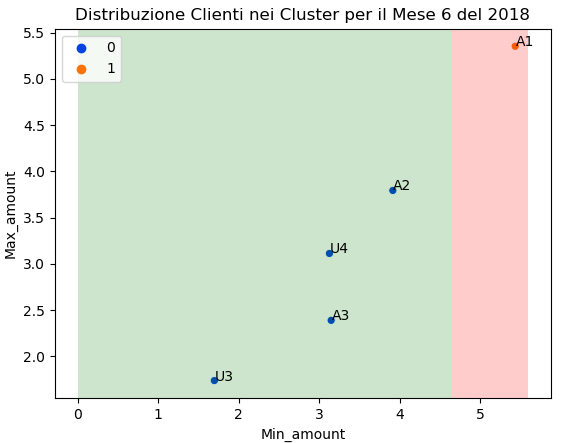
\includegraphics[width=0.8\textwidth]{6_2018.png}
    \centering
    \caption{Distribuzione dei Clienti per il Mese 6 del 2018}
    \label{fig:challenge}
\end{figure}

\noindent Il \textit{Decision Tree Classifier} a cui viene dato come input l'intero dataset del $6/2018$ produce il seguente albero con le seguenti regole riportate in scala reale (sinistra) e in scala logaritmica (destra). 
\vspace{0.2cm}

\begin{center}
\begin{minipage}{5cm}
\begin{Verbatim}[t][fontsize=\small, frame=single]
|--- Min_amount <= 4.64
|   |--- class: 0
|--- Min_amount >  4.64
|   |--- class: 1
\end{Verbatim}
\end{minipage}
\end{center}
\vspace{0.5cm}
\begin{minipage}{8cm}
\raggedright
\begin{Verbatim}[t][fontsize=\small, frame=single]
Rule 1
Rule: Min_amount <= 43294.397
Rule 2
Rule: Min_amount > 43294.397
\end{Verbatim}
\end{minipage}%
\begin{minipage}{6cm}
\raggedleft
\begin{Verbatim}[t][fontsize=\small, frame=single]
Rule 1
Rule: Min_amount <= 4.636
Rule 2
Rule: Min_amount > 4.636
\end{Verbatim}
\end{minipage}

\vspace{0.9cm}

\noindent Dai dati ricavati è possibile identificare nella regola $2$ l'anomalia che è possibile visualizzare nella figura \ref{fig:challenge}, essa si verifica quando \verb{Min_amount > 4.64{ (scala logaritmica in base dieci) oppure \verb{Min_amount > 43294.397{ (scala reale).

\noindent Dopo aver completato la ricerca di eventuali anomalie statiche per ogni mese del piccolo dataset reale, avendo a disposizione un arco temporale di diversi mesi, è stata condotta una breve analisi dinamica dei dati raccolti. 

Sono state quindi analizzate il numero di volte in cui un utente effettuava un cambio di cluster e le segnalazioni di anomalia nei mesi considerati. I cluster di appartenenza di ogni cliente nell'arco temporale sono riportati nella tabella \ref{tab:dinamiche}, dove il numero di cluster parte da $0$ fino ad un massimo di $2$ (quindi massimo $3$ cluster all'interno di un mese) e nel caso in cui non venga riportato nessun cluster il cliente in quel mese non ha effettuato transazioni.

\begin{table}[ht]
\centering
\begin{tabular}{|r||c|c|c|c|c|c|c|c|} \hline
Label & $1/2018$ & $2/2018$& $3/2018$ & $4/2018$ & $5/2018$ & $6/2017$ &$7/2018$ &$8/2018$\\ \hline
A1 & 0 & 0 & 0 & 2 & 0 & 1& 1 & 1 \\ \hline
U1 &  &  & 0   &   &   &  &   & \\ \hline
U2 &  &  & 0   &   &   &  &   & \\ \hline
A2 & 1 & 0 & 1 & 0 & 0 & 0& 0 &1 \\ \hline
U3 & 0 & 0 & 0 & 0 & 0 & 0& 0&0\\ \hline
A3 & 0 & 1 & 0 & 1 & 0 & 0& 1 &1\\ \hline
U4 & 0 & 0 & 0 & 0 & 1 & 0& 1&0\\ \hline
\end{tabular}
\caption{Composizione mensile dei cluster}
\label{tab:dinamiche}
\end{table}

\noindent Nella tabella \ref{tab:dinamiche} sopra riportata è possibile analizzare varie casistiche di distribuzione dei cluster, ad esempio andando a considerare l'utente \verb{U3{ è possibile notare come rimanga costante la sua presenza nel cluster $0$ e non effettui mai salti di cluster.  Un cliente che è possibile notare particolarmente anomalo è\verb{ A3 {che effettua numerosi cambiamenti di cluster e si posiziona come anomalo in cinque mesi su otto. Durante il mese $7/2018$ non viene considerato anomalo in quanto si muove con l'utente\verb{ U4{ con cui forma una sotto popolazione che parte dal cluster 0 per spostarsi nel 1. 

 Vengono segnalate come anomalie statiche rispettivamente:  il cliente\verb{ A2 {per il mese $1/2018$, il cliente\verb{ A3 {per il mese $2/2018$, il cliente\verb{ A2 {per il mese $3/2018$, il cliente\verb{ A1 {e \verb{A3{ per il mese $4/2018$, il cliente\verb{ U4 {per il mese $5/2018$ e il cliente\verb{ A1 {per il mese $6/2018$. 

Inoltre, è possibile notare che all'interno di uno stesso mese ($8/2018$) possono esserci più cluster ma nessuna anomalia di tipo statico, ed allo stesso tempo presentare un anomalia di tipo dinamico con il mese precedente ($7/2018$) anch'esso privo di anomalie statiche.

\section{Considerazioni}

Analizzando i risultati ottenuti applicando l'approccio proposto nel Capitolo $4$ al dataset della challenge Kaggle e al piccolo dataset reale possiamo vedere che è sempre possibile identificare utenti anomali all'interno di un mese o un periodo di tempo, nel caso in cui essi siano presenti. Infatti, in entrambi i dataset vengono trovate varie anomalie, con la differenza che nella challenge avendo un numero estremamente superiore di clienti si è potuto riscontrare un numero superiore di cluster e di utenti anomali.

La numerosità del campione considerato va inoltre ad influire sulla generazione delle regole per le anomalie. Per questo motivo, nel caso dei risultati provenienti dal dataset reale a seguito dell'applicazione del \textit{Decision Tree Classifier} risultava sufficiente esprimere la regola in funzione di un solo attributo, questo non accade invece nell'esempio riportato per la challenge dove risulta necessario l'impiego di due metriche per poter dare una spiegazione completa delle anomalie. 

 I soli risultati ottenuti dall'analisi focalizzata su un solo mese non sono però sufficienti a determinare su un utente sia effettivamente fraudolento. Per questo motivo è necessario implementare parallelamente a questa analisi un'analisi longitudinale su un lasso di tempo più o meno breve per investigare cosa quel utente abbia fatto nei mesi precedenti e successivi a quello considerato. 

%Approfondendo il suo comportamento e tracciandone un profilo che spieghi i suoi posizionamenti anomali nel periodo considerato, per ottenere dei dati più precisi che permettano di distinguere tra un comportamento plausibile ed uno sospetto. 
Non è sufficiente un singolo posizionamento anomalo o un singolo salto di cluster per avere la certezza di aver identificato un utente fraudolento, perché questi comportamenti posso essere facilmente influenzabili da agenti esterni (come festività o periodo fiscali) e non essere indice di attività malevola.

Eseguire quindi un analisi che comprenda sia un analisi statica che una dinamica porta ad avere un analisi discretamente completa del comportamento di un utente nel periodo considerato. In modo tale che, nel momento in cui tali analisi e segnalazioni pervengano all'operatore designato di analizzarle, esso possa eseguire il compito nel modo più corretto possibile avendo lui a disposizione tutti i dati necessari.
























